\chapter{对超新星遗迹W51C的磁流体模拟及观测分析}
\label{W51C}



\section{研究历史及意义}
\label{W51Cintro}
SNR W51C存在于W51复合区中,除了这个遗迹,这个区域还包括两个电离氢区W51 A/B。
这两个电离氢区尺寸都很大,而且包括很多小一些的电离结构,比如G49.2-0.35。
SNR W51C有很厚的半圆形的单壳层,射电图像尺寸大约为14\am $\times$ 20\am
\citep{Copetti1991,Subrahmanyan1995}。
而且SNR W51C一侧与电离氢区W51B相邻,最近的观测显示在此处有明显的高能特征
\citep{Abdo2009,Aleksic2012},因此我们认为这个遗迹是与分子云相互作用的。
在W51B的东侧,也就是临近W51C的爆发中心,我们探测到了OH的1720MHz脉泽
\citep{Hewitt2008,Brogan2013},这是支持相互作用的另一个证据。
W51A是一个活跃的恒星形成区,但是并没有任何迹象表明与W51C相关,不过和W51B在
一氧化碳(CO)和红外图像上看是互相关联的\citep{Kang2010,Parsons2012,Ginsburg2015}。
两个电离氢区的距离是5 kpc $\sim$ 8 kpc
\citep{Genzel1981,Schneps1981,Xu2009,Sato2010,Tian2013},而SNR W51C的距离是
4.3 kpc \citep{Tian2013} 到 6 kpc \citep{Koo1995}。
这三者的空间关系让我们思考是否它们也有一定物理联系。

之前对这个复合体的观测已经有很多,可是其中主体结构之间的联系依然不清楚。
因此,为了研究遗迹和电离氢区的物理联系,我们决定模拟这个遗迹的磁流体演化,并通过分析
射电偏振数据和OH谱线数据来理解模拟的结果。

\section{数据处理}
\label{W51Cdata}

\subsection{偏振数据处理}
\label{W51Cpoldata}
我们使用的偏振数据来源于Effelsberg 11cm (2.695GHz) 巡天\citep{1999A&A...350..447D}。
这个巡天其实已经展示了W51复合区的偏振图像,可是他们为了图像可以覆盖
更大片区域,使用了较低的分辨率,从而导致一些小结构模糊不清。
原本的分辨率是5\am, 实际展示的是12\am。
在图~\ref{fig:mag}中

\begin{figure*}
   \centering
   \includegraphics[width=0.495\textwidth]{mag0.eps}
   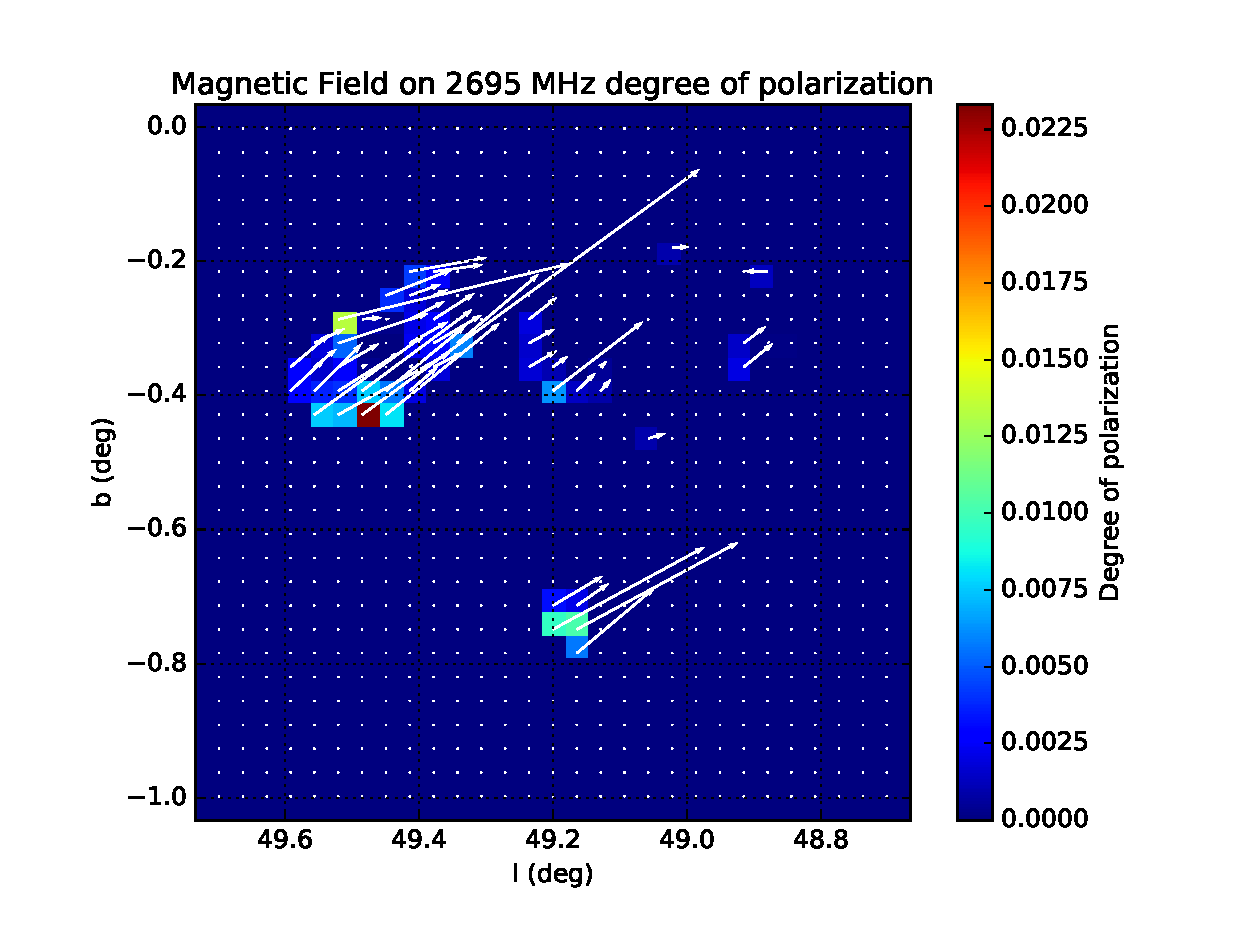
\includegraphics[width=0.495\textwidth]{modi_mag.eps}
   \caption{左侧图像中,彩色背景是1.4GHz的来自VGPS的连续谱图像,黑色的箭头代表磁场,箭头
   长度代表偏振强度(mK),最强处为1581mK,箭头方向代表磁场方向。
   右侧图像中彩色背景是在2695MHz处的偏振度,白色的箭头代表磁场,箭头
   长度代表偏振度,最强处为$2\%$,箭头方向代表磁场方向。
   }
\label{fig:mag}
\end{figure*}


\section{射电偏振分析}
\section{羟基谱线分析}
\section{讨论}
